\documentclass[crop, tikz]{standalone}
\usepackage{tikz}
\usepackage{pgfplots}
\usepackage{amsbsy}

\usetikzlibrary{automata, chains, decorations.pathmorphing, positioning}

\definecolor{echodrk}{HTML}{0099cc}

\begin{document}
\begin{tikzpicture} [scale=1.3, every node/.style={transform shape},start chain=1 going right, start chain=2 going right]

	\node[state, fill=red!20, on chain=1, very thick, text depth=0pt] (1) {$s_0$};
	\node[state, fill=red!20, on chain=1, very thick, text depth=0pt] (2) {$s_1$};
	\node[state, fill=red!20, on chain=1, very thick, text depth=0pt] (3) {$s_2$};
	\node[on chain=1] (md) {\dots};
	\node[state, fill=red!20, on chain=1, very thick, text depth=0pt] (n) {$s_n$};
	\draw[>=stealth, color=red, text=black, very thick, auto=right,loop above/.style={out=75,in=105,loop}, every loop]
		(1) edge node[above] {\footnotesize$\boldsymbol \omega_{11}$} (2)
		(2) edge node[above] {\footnotesize$\boldsymbol \omega_{11}$} (3)
		(3) edge node[above] {\footnotesize$\boldsymbol \omega_{11}$} (md)
		(md) edge node[above] {\footnotesize$\boldsymbol \omega_{11}$} (n);
					
	\node[rectangle, thick, fill=red!20, draw] at (-2, 1.7) (y1) {$id_0$};
	\node[rectangle, thick, fill=red!20, draw] at (0, 1.7) (y2) {$id_1$};
	\node[rectangle, thick, fill=red!20, draw] at (2, 1.7) (y3) {$id_2$};
	\node at (4, 1.7) (ymd) {\dots};
	\node[rectangle, thick, fill=red!20, draw] at (6, 1.7) (yn) {$id_n$};
				
	\draw[-stealth, color=red, text=black, very thick, dashed]
		(1) edge node[right] {${\bf O'}_{0,id_0}^1$} (y1)
		(2) edge node[right] {${\bf O'}_{1,id_1}^1$} (y2)
		(3) edge node[right] {${\bf O'}_{2,id_2}^1$} (y3)
		(n) edge node[right] {${\bf O'}_{n,id_n}^1$} (yn);
				
	\node[rectangle, fill=red!20, draw, scale=0.2, minimum size=20em,above = 2cm of y1] at (-1, 2) (gauss1) {
		\begin{tikzpicture}
			\begin{axis}[axis lines=none, ticks=none,xmax=3, xmin=-3,ymax=1.1]
				\addplot[ultra thick,black, no markers,samples=200] {exp(-x^2)};
			\end{axis}
		\end{tikzpicture}
	};

	\node[rectangle, fill=red!20, draw, scale=0.2, minimum size=20em,above = 2cm of y2] at (1, 2) (gauss2) {
		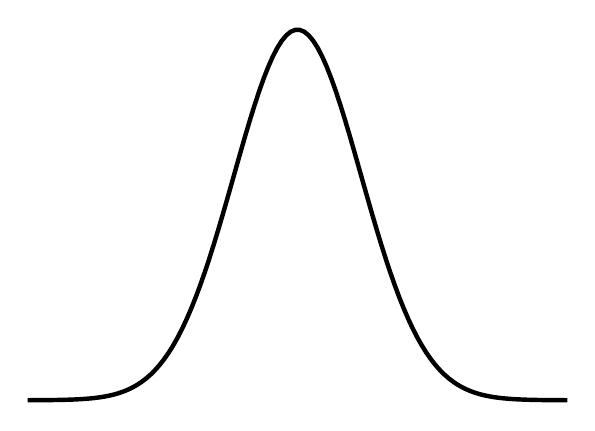
\begin{tikzpicture}
			\begin{axis}[axis lines=none, ticks=none,xmax=3, xmin=-3,ymax=1.1]
				\addplot[ultra thick,black, no markers,samples=200] {exp(-x^2)};
			\end{axis}
		\end{tikzpicture}
	};

	\node[rectangle, fill=red!20, draw, scale=0.2, minimum size=20em,above = 2cm of y3] at (3, 2) (gauss3) {
		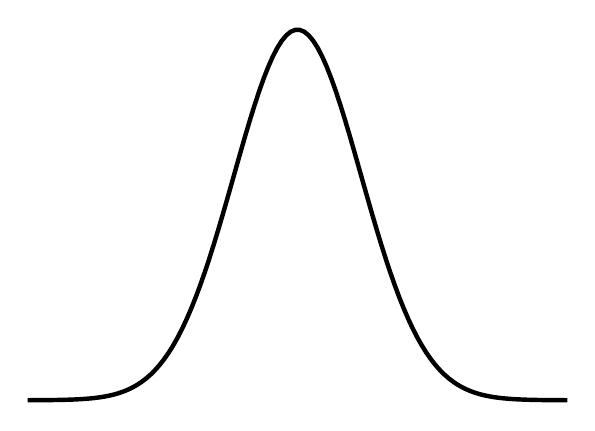
\begin{tikzpicture}
			\begin{axis}[axis lines=none, ticks=none,xmax=3, xmin=-3,ymax=1.1]
				\addplot[ultra thick,black, no markers,samples=200] {exp(-x^2)};
			\end{axis}
		\end{tikzpicture}
	};
				
	\node at (5, 4.7) (gaussmd) {\dots};
				
	\node[rectangle, fill=red!20, draw, scale=0.2, minimum size=20em,above = 2cm of yn] at (7, 2) (gaussn) {
		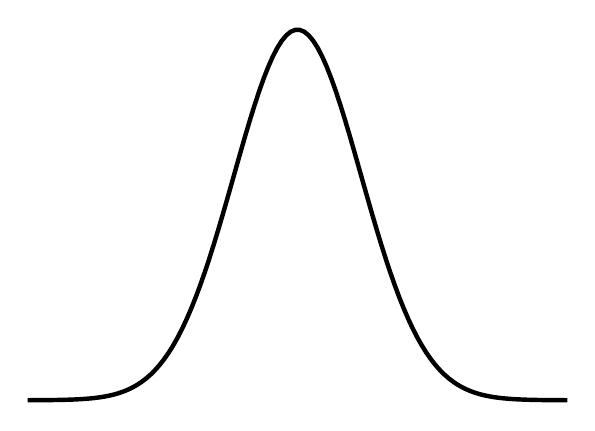
\begin{tikzpicture}
			\begin{axis}[axis lines=none, ticks=none,xmax=3, xmin=-3,ymax=1.1]
				\addplot[ultra thick,black, no markers,samples=200] {exp(-x^2)};
			\end{axis}
		\end{tikzpicture}
	};
				
	\draw[-stealth, color=red, text=black, very thick, dotted]
		(y1) edge node[left] {$\mu_{id_0}^1$} node[right] {$\sigma_{id_0}^1$} (gauss1)
		(y2) edge node[left] {$\mu_{id_1}^1$} node[right] {$\sigma_{id_1}^1$} (gauss2)
		(y3) edge node[left] {$\mu_{id_2}^1$} node[right] {$\sigma_{id_2}^1$} (gauss3)
		(yn) edge node[left] {$\mu_{id_n}^1$} node[right] {$\sigma_{id_n}^1$} (gaussn);
	%%%%%% BOUNDARY %%%%%%%
					
	%%%%%% BOUNDARY %%%%%%%
	\node[state, fill=echodrk!20, on chain=2, very thick, text depth=0pt] (21) at (0, -2) {$s_0$};
	\node[state, fill=echodrk!20, on chain=2, very thick, text depth=0pt] (22) {$s_1$};
	\node[state, fill=echodrk!20, on chain=2, very thick, text depth=0pt] (23) {$s_2$};
	\node[on chain=2] (2md) {\dots};
	\node[state, fill=echodrk!20, on chain=2, very thick, text depth=0pt] (2n) {$s_n$};
	\draw[>=stealth, color=blue, text=black, very thick, auto=right,loop above/.style={out=75,in=105,loop}, every loop]
		(21) edge node[below] {\footnotesize$\boldsymbol \omega_{22}$} (22)
		(22) edge node[below] {\footnotesize$\boldsymbol \omega_{22}$} (23)
		(23) edge node[below] {\footnotesize$\boldsymbol \omega_{22}$} (2md)
		(2md) edge node[below] {\footnotesize$\boldsymbol \omega_{22}$} (2n);
					
	\node[rectangle, thick, fill=echodrk!20, draw] at (-2, -3.7) (2y1) {$id_0$};
	\node[rectangle, thick, fill=echodrk!20, draw] at (0, -3.7) (2y2) {$id_1$};
	\node[rectangle, thick, fill=echodrk!20, draw] at (2, -3.7) (2y3) {$id_2$};
	\node at (4, -3.7) (2ymd) {\dots};
	\node[rectangle, thick, fill=echodrk!20, draw] at (6, -3.7) (2yn) {$id_n$};
				
	\draw[-stealth, color=blue, text=black, very thick, dashed]
		(21) edge node[right] {${\bf O'}_{0,id_0}^2$} (2y1)
		(22) edge node[right] {${\bf O'}_{1,id_1}^2$} (2y2)
		(23) edge node[right] {${\bf O'}_{2,id_2}^2$} (2y3)
		(2n) edge node[right] {${\bf O'}_{n,id_n}^2$} (2yn);
				
	\node[rectangle, fill=echodrk!20, draw, scale=0.2, minimum size=20em,above = 2cm of 2y1] at (-1, -9.5) (2gauss1) {
		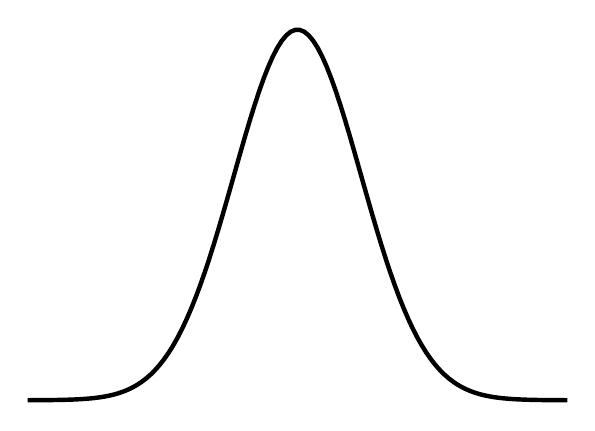
\begin{tikzpicture}
			\begin{axis}[axis lines=none, ticks=none,xmax=3, xmin=-3,ymax=1.1]
				\addplot[ultra thick,black, no markers,samples=200] {exp(-x^2)};
			\end{axis}
		\end{tikzpicture}
	};

	\node[rectangle, fill=echodrk!20, draw, scale=0.2, minimum size=20em,above = 2cm of 2y2] at (1, -9.5) (2gauss2) {
		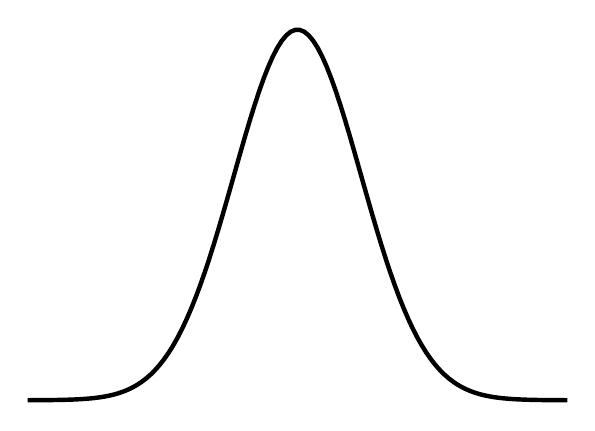
\begin{tikzpicture}
			\begin{axis}[axis lines=none, ticks=none,xmax=3, xmin=-3,ymax=1.1]
				\addplot[ultra thick,black, no markers,samples=200] {exp(-x^2)};
			\end{axis}
		\end{tikzpicture}
	};

	\node[rectangle, fill=echodrk!20, draw, scale=0.2, minimum size=20em,above = 2cm of 2y3] at (3, -9.5) (2gauss3) {
		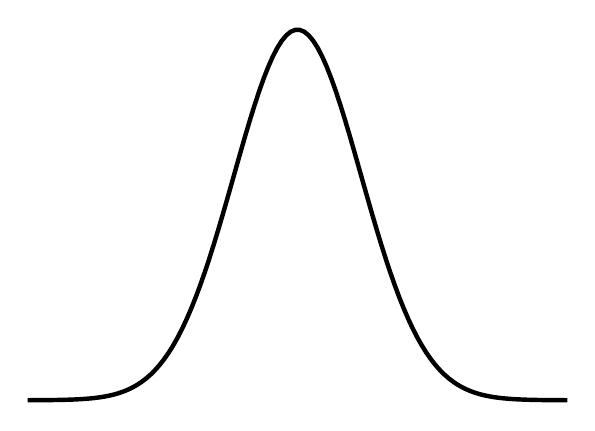
\begin{tikzpicture}
			\begin{axis}[axis lines=none, ticks=none,xmax=3, xmin=-3,ymax=1.1]
				\addplot[ultra thick,black, no markers,samples=200] {exp(-x^2)};
			\end{axis}
		\end{tikzpicture}
	};
				
	\node at (5, -6.8) (2gaussmd) {\dots};
				
	\node[rectangle, fill=echodrk!20, draw, scale=0.2, minimum size=20em,above = 2cm of 2yn] at (7, -9.5) (2gaussn) {
		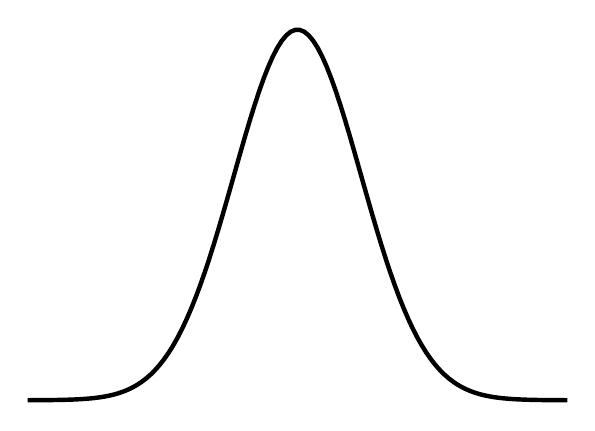
\begin{tikzpicture}
			\begin{axis}[axis lines=none, ticks=none,xmax=3, xmin=-3,ymax=1.1]
				\addplot[ultra thick,black, no markers,samples=200] {exp(-x^2)};
			\end{axis}
		\end{tikzpicture}
	};
				
	\draw[-stealth, color=blue, text=black, very thick, dotted]
		(2y1) edge node[left] {$\mu_{id_0}^2$} node[right] {$\sigma_{id_0}^2$} (2gauss1)
		(2y2) edge node[left] {$\mu_{id_1}^2$} node[right] {$\sigma_{id_1}^2$} (2gauss2)
		(2y3) edge node[left] {$\mu_{id_2}^2$} node[right] {$\sigma_{id_2}^2$} (2gauss3)
		(2yn) edge node[left] {$\mu_{id_n}^2$} node[right] {$\sigma_{id_n}^2$} (2gaussn);	
					
	%%%% COMBO %%%%%
	\draw[-stealth, very thick, auto=right,decoration={snake, segment length=2mm, amplitude=0.5mm,post length=1.5mm}]
		(1) edge[decorate] node[left, near start] {\footnotesize$\boldsymbol \omega_{12}$} (22)
		(2) edge[decorate] node[left, near start] {\footnotesize$\boldsymbol \omega_{12}$} (23)
		(3) edge[decorate] node[left, near start] {\footnotesize$\boldsymbol \omega_{12}$} (2md)
		(md) edge[decorate] node[left, near start] {\footnotesize$\boldsymbol \omega_{12}$} (2n);
	
	\draw[-stealth, very thick, auto=right,decoration={snake, segment length=2mm, amplitude=0.5mm,post length=1.5mm}]
		(21) edge[decorate] node[left, near start] {\footnotesize$\boldsymbol \omega_{21}$} (2)
		(22) edge[decorate] node[left, near start] {\footnotesize$\boldsymbol \omega_{21}$} (3)
		(23) edge[decorate] node[left, near start] {\footnotesize$\boldsymbol \omega_{21}$} (md)
		(2md) edge[decorate] node[left, near start] {\footnotesize$\boldsymbol \omega_{21}$} (n);
				
	%%%% START STATES %%%%%
	\node[text depth=0pt] at (-2, -1) (S) {start};
	
	\draw[-stealth, very thick, auto=right,decoration={snake, segment length=2mm, amplitude=0.5mm,post length=1.5mm}]
		(S) edge[decorate] node[above] {\footnotesize$\pi_1$} (1)
		(S) edge[decorate] node[below] {\footnotesize$\pi_2$} (21);
\end{tikzpicture}
\end{document}
